\documentclass[11pt,tikz]{standalone}
\usepackage[OT1]{eulervm}
\usepackage{libertine}

%\usepackage{amsmath,amssymb}

\usetikzlibrary{positioning,calc}

% ------------------- %
% Various tikz styles %
% ------------------- %

\tikzset{
  contraction/.style={
    line width=.8pt,
    ColourBase
  },
  inline math/.style={
    baseline = .5ex,
    every node/.style = {anchor=south, text depth=0.35ex, inner sep=1pt}
  },
}

% ------------ %
% graph styles %
% ------------ %

\tikzset{
  graph style/.style={
    baseline={([yshift=-.5ex]current bounding box.center)},
    node distance=.5,
  },
  skeleton node/.style={
    black,fill,circle,inner sep=0pt,minimum size=3.5pt
  },
  skeleton bond/.style={
    draw,
  },
}

% ----------- %
% Node styles %
% ----------- %

\tikzset{
  inner/.style={
    fill=#1,
    circle,
    inner sep=0pt,
    minimum size=3.5pt
  },
  outer/.style={
    draw=#1,
    thick, circle,
    inner sep=0pt,
    minimum size=6pt,
  },
  outerouter/.style={
    draw=#1,
    thick, circle,
    inner sep=0pt,
    minimum size=9.5pt,
  },
  inner 1/.style={
    inner=ColourBase,
  },
  inner 2/.style={
    inner=ColourHl1,
  },
  inner 3/.style={
    inner=ColourHl2,
  },
  outer 1/.style={
    outer=ColourBase,
  },
  outer 2/.style={
    outer=ColourHl1,
  },
  outer 3/.style={
    outer=ColourHl2,
  },
  outerouter 1/.style={
    outerouter=ColourBase,
  },
  outerouter 2/.style={
    outerouter=ColourHl1,
  },
  outerouter 3/.style={
    outerouter=ColourHl2,
  },
}

% ----------- %
% Bond styles %
% ----------- %

\tikzset{
  bond default/.style={
    skeleton bond,
    line width=1.2pt,
  },
  bond 1/.style={
    bond default,
    ColourBase,
  },
  bond 2/.style={
    bond default,
    ColourHl1,
  },
  bond 3/.style={
    bond default,
    ColourHl2,
  },
}

% ------------------------------------------- %
% position function                           %
% http://tex.stackexchange.com/a/102266/39313 %
% ------------------------------------------- %

\makeatletter
\tikzset{
  position/.style args={#1 degrees from #2}{
    at=(#2.#1), anchor=#1+180, shift=(#1:\tikz@node@distance)
  }
}
\makeatother

% ------- %
% Colours %
% ------- %

% Playroom colour scheme
% http://www.colourlovers.com/palette/1047246/Playroom
\definecolor{PeelingPaper}{RGB}{5,135,137}
\definecolor{WoodenPlatforms}{RGB}{80,61,46}
\definecolor{Puzzle24000}{RGB}{213,75,26}
\definecolor{Escape}{RGB}{227,167,47}

%% u.make.me.happy colour scheme
%% http://www.colourlovers.com/palette/360922/u.make.me.happy
%\definecolor{Amelllatoo}{HTML}{5CACC4}
%\definecolor{Lmao}{HTML}{8CD19D}
%\definecolor{UFunny}{HTML}{CEE879}
%\definecolor{FairyStream}{HTML}{FCB653}
%\definecolor{Hexy}{HTML}{FF5254}

%% Mongo for Mormons colour scheme
%% http://www.colourlovers.com/palette/324775/Mangos_for_Mormons
%\definecolor{Murky}{HTML}{595643}
%\definecolor{Everything}{HTML}{4E6B66}
%\definecolor{Melon}{HTML}{ED834E}
%\definecolor{TheHolyGrail}{HTML}{EBCC6E}

%% Chick Mellow colour scheme
%% http://www.colourlovers.com/palette/254301/[Chic]_-_Mellow
%\definecolor{Gemma}{HTML}{11644D}
%\definecolor{MellowMeadow}{HTML}{A0B046}
%\definecolor{TheKingsCrown}{HTML}{F2C94E}
%\definecolor{MellowMe}{HTML}{F78145}
%\definecolor{AlmostZeroZero}{HTML}{F24E4E}

% Other colours I use
\definecolor{Tropiteal}{RGB}{0,168,198}
\definecolor{TealDrop}{RGB}{64,192,203}
\definecolor{WhiteTrash}{RGB}{249,242,231}
\definecolor{AtomicBikini}{RGB}{174,226,57}
\definecolor{FeebleWeek}{RGB}{143,190,0}
\definecolor{ICantExpress}{RGB}{28,20,13}
\definecolor{Marty}{RGB}{250,42,0}
\definecolor{WeddedPassion}{RGB}{164,7,120}


\colorlet{ColourBase}{PeelingPaper}
\colorlet{ColourHl1}{Puzzle24000}
\colorlet{ColourHl2}{FeebleWeek}
\colorlet{ColourHl3}{Escape}
\colorlet{ColourDark}{WoodenPlatforms}
\colorlet{ColourDark2}{WeddedPassion}

\newcommand{\ColBaseText}{blue}
\newcommand{\ColHlIText}{red}



\begin{document}
  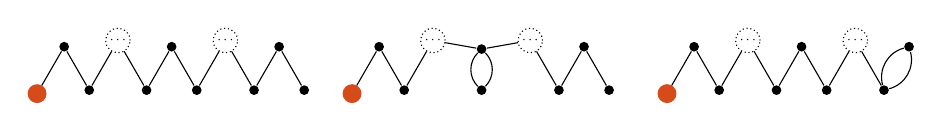
\begin{tikzpicture}[graph style]
    \begin{scope}
      \node[outer 2, fill=ColourHl1] (n1) {};
      \node[skeleton node] (n2) [position=60 degrees from n1] {}
        edge[skeleton bond] (n1);
      \node[skeleton node] (n3) [position=300 degrees from n2] {}
        edge[skeleton bond] (n2);
      \node[inner sep=2pt,circle,draw,thin,densely dotted] (n4) [position=60 degrees from n3] [scale=0.5] {$\cdots$}
        edge[skeleton bond] (n3);
      \node[skeleton node] (n5) [position=300 degrees from n4] {}
        edge[skeleton bond] (n4);
      \node[skeleton node] (n6) [position=60 degrees from n5] {}
        edge[skeleton bond] (n5);
      \node[skeleton node] (n7) [position=300 degrees from n6] {}
        edge[skeleton bond] (n6);
      \node[inner sep=2pt,circle,draw,thin,densely dotted] (n8) [position=60 degrees from n7] [scale=0.5] {$\cdots$}
        edge[skeleton bond] (n7);
      \node[skeleton node] (n9) [position=300 degrees from n8] {}
        edge[skeleton bond] (n8);
      \node[skeleton node] (n10) [position=60 degrees from n9] {}
        edge[skeleton bond] (n9);
      \node[skeleton node] (n11) [position=300 degrees from n10] {}
        edge[skeleton bond] (n10);
    \end{scope}
    \begin{scope}[xshift=4cm]
      \node[outer 2, fill=ColourHl1] (n1) {};
      \node[skeleton node] (n2) [position=60 degrees from n1] {}
        edge[skeleton bond] (n1);
      \node[skeleton node] (n3) [position=300 degrees from n2] {}
        edge[skeleton bond] (n2);
      \node[inner sep=2pt,circle,draw,thin,densely dotted] (n4)
        [position=60 degrees from n3] [scale=0.5] {$\cdots$}
        edge[skeleton bond] (n3);
      \node[skeleton node] (n5) [node distance=.4,position=350 degrees from n4] {}
        edge[skeleton bond] (n4);
      \node[skeleton node] at (n3 -| n5) {}
        edge[skeleton bond,bend right=45] (n5)
        edge[skeleton bond,bend left=45]  (n5);
      \node[inner sep=2pt,circle,draw,thin,densely dotted] (n8)
        [node distance=.4,position=10 degrees from n5] [scale=0.5] {$\cdots$}
        edge[skeleton bond] (n5);
      \node[skeleton node] (n9) [position=300 degrees from n8] {}
        edge[skeleton bond] (n8);
      \node[skeleton node] (n10) [position=60 degrees from n9] {}
        edge[skeleton bond] (n9);
      \node[skeleton node] (n11) [position=300 degrees from n10] {}
        edge[skeleton bond] (n10);
    \end{scope}
    \begin{scope}[xshift=8cm]
      \node[outer 2, fill=ColourHl1] (n1) {};
      \node[skeleton node] (n2) [position=60 degrees from n1] {}
        edge[skeleton bond] (n1);
      \node[skeleton node] (n3) [position=300 degrees from n2] {}
        edge[skeleton bond] (n2);
      \node[inner sep=2pt,circle,draw,thin,densely dotted] (n4) [position=60 degrees from n3] [scale=0.5] {$\cdots$}
        edge[skeleton bond] (n3);
      \node[skeleton node] (n5) [position=300 degrees from n4] {}
        edge[skeleton bond] (n4);
      \node[skeleton node] (n6) [position=60 degrees from n5] {}
        edge[skeleton bond] (n5);
      \node[skeleton node] (n7) [position=300 degrees from n6] {}
        edge[skeleton bond] (n6);
      \node[inner sep=2pt,circle,draw,thin,densely dotted] (n8) [position=60 degrees from n7] [scale=0.5] {$\cdots$}
        edge[skeleton bond] (n7);
      \node[skeleton node] (n9) [position=300 degrees from n8] {}
        edge[skeleton bond] (n8);
      \node[skeleton node] (n10) [position=60 degrees from n9] {}
        edge[skeleton bond, bend right=45] (n9)
        edge[skeleton bond, bend left=45]  (n9);
    \end{scope}
  \end{tikzpicture}
\end{document}
